\title{Opgave 164 \\ \small e16g3113}
\date{\today}
\documentclass[12pt]{article}

\usepackage{amsmath}
\usepackage{amssymb}
\usepackage{amsthm}
\usepackage[
%  disable, %turn off todonotes
 colorinlistoftodos, %enable a coloured square in the list of todos
 textwidth=\marginparwidth, %set the width of the todonotes
 textsize=scriptsize, %size of the text in the todonotes
 ]{todonotes}
\usepackage{tikz}

\usepackage[utf8]{inputenc}
\usepackage[danish,english]{babel}
\renewcommand\qedsymbol{$\blacksquare$}

\begin{document}

\begin{figure}
\centering
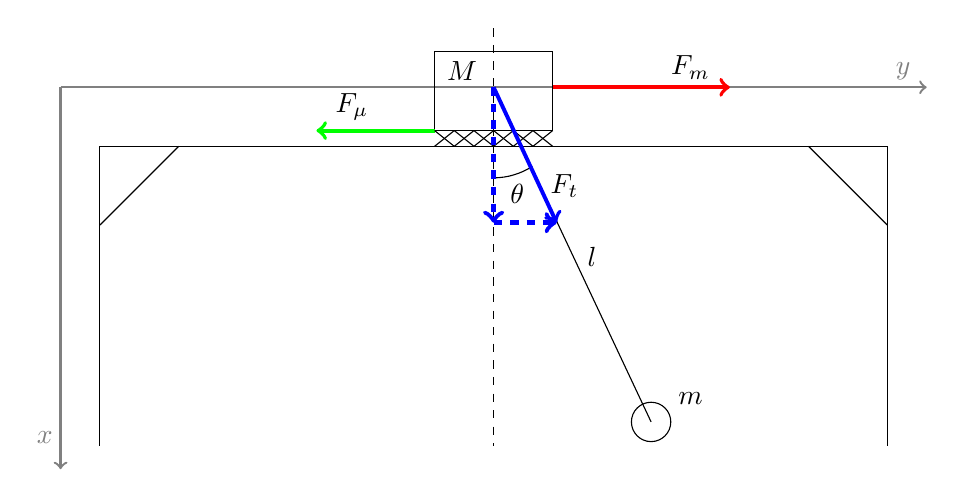
\begin{tikzpicture}
%ramme
\draw (-5,0)--(-5,-3.8);
\draw (-2,0)--(-4,0);
\draw (-5,0)--(5,0);
\draw (5,0)--(5,-3.8);
\draw [dashed](0,1.5)--(0,-3.8);
\draw (-5,-1)--(-4,0);
\draw (5,-1)--(4,0);
%akser
\draw[->,line width=0.3 mm, gray] (-5.5,0.75)--(5.5,0.75);
\draw[->,line width=0.3 mm, gray] (-5.5,0.75)--(-5.5,-4.1);
\node [gray]at(-5.7,-3.7) {$x$};
\node [gray]at(5.2,0.95) {$y$};
%slæde 
\draw (-0.75,0.2)rectangle (0.75,1.2);
\node at(-0.4,0.95) {$M$};
\draw[->,line width=0.5 mm, red] (0.75,0.75)--(3,0.75);
\node at(2.5,1) {$F_m$};
\draw[->,line width=0.5 mm, green] (-0.75,0.2)--(-2.25,0.2);
\node at(-1.8,0.5) {$F_{\mu}$};
\node at(1.25,-1.4) {$l$};
%friktion
\draw (-0.75,0.2)--(-0.50,0);
\draw (-0.75,0)--(-0.50,0.2);
\draw (-0.50,0)--(-0.25,0.2);
\draw (-0.50,0.2)--(-0.25,0);
\draw (-0.25,0)--(0,0.2);
\draw (-0.25,0.2)--(0,0);
\draw (0.75,0.2)--(0.50,0);
\draw (0.75,0)--(0.50,0.2);
\draw (0.50,0)--(0.25,0.2);
\draw (0.50,0.2)--(0.25,0);
\draw (0.25,0)--(0,0.2);
\draw (0.25,0.2)--(0,0);
%pendul
\draw (0,0.75)--(2,-3.5);
\draw (2,-3.5)circle[radius=0.25];
\draw (0,-0.4) arc (-90:-57:0.9);
\node at(0.3,-0.6) {$\theta$};
\node at(2.5,-3.2) {$m$};
\draw[->,line width=0.5 mm, blue] (0,0.75)--(0.8,-0.97);
\node at(0.9,-0.5) {$F_t$};
\draw[dashed,->,line width=0.6 mm, blue] (0,0.75)--(0,-0.97);
\draw[dashed,->,line width=0.6 mm, blue] (0,-0.97)--(0.8,-0.97);
%pendul
%\draw (0,0.75)--(2,-3.5);
%\draw (2,-3.5)circle[radius=0.25];
%\draw (0,-0.4) arc (-90:-57:0.9);
%\node at(0.3,-0.6) {$\theta$};
%\draw[->,line width=0.5 mm, blue] (2,-3.5)--(0.4,-4.25);
%\node at(0.9,-3.7) {$F_k$};
%\draw[->,line width=0.5 mm, blue] (2,-3.5)--(2,-5.3);
%\node at(2.5,-4.9) {$F_g$};
%\node at(2.5,-3.2) {$m$};
%\node at(1.8,-2.3) {$F_t$};
%\draw[->,line width=0.5 mm, blue] (2,-3.5)--(1.25,-1.89);
\end{tikzpicture}
\end{figure}
%
\begin{figure}
\centering
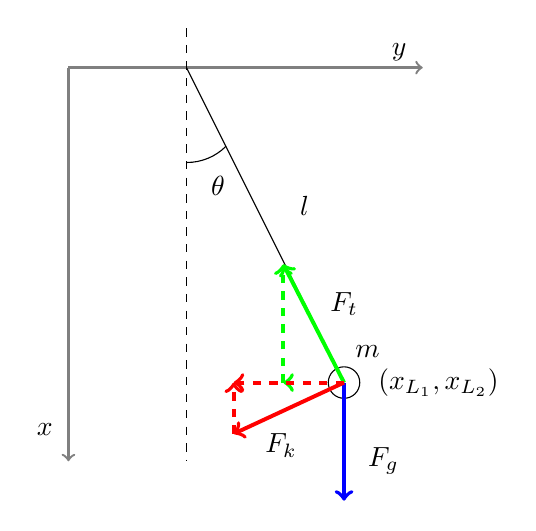
\begin{tikzpicture}
%akser 
\draw[->,line width=0.3 mm, gray] (-1.5,0)--(3,0);
\draw[->,line width=0.3 mm, gray] (-1.5,0)--(-1.5,-5);
\draw (0,0)--(2,-4);
\draw (2,-4)circle[radius=0.2];
\node at(1.5,-1.75) {$l$};
\node at(2.3,-3.6) {$m$};
\node at(3.2,-4) {$(x_{L_1},x_{L_2})$};
\draw [dashed](0,0.5)--(0,-5);
\draw (0.5,-1)arc[radius=0.7,start angle=-45,end angle=-90];
\node at(0.4,-1.5){$\theta$};
%pile
\draw[->,line width=0.5 mm,green] (2,-4)--(1.23,-2.5);
\draw[dashed,->,line width=0.5 mm,green] (2,-4)--(1.23,-4);
\draw[dashed,->,line width=0.5 mm,green] (1.23,-4)--(1.23,-2.5);
\node at(2,-3) {$F_t$};
\draw[->,line width=0.5 mm,blue] (2,-4)--(2,-5.5);
\node at(2.5,-5) {$F_g$};
\draw[->,line width=0.5 mm,red] (2,-4)--(0.6,-4.65);
\draw[dashed,->,line width=0.5 mm,red] (2,-4)--(0.6,-4);
\draw[dashed,->,line width=0.5 mm,red] (0.6,-4.65)--(0.6,-4);
\node at(1.2,-4.8) {$F_k$};
\node at(-1.8,-4.6) {$x$};
\node at(2.7,0.2) {$y$};
\end{tikzpicture}
\label{fig:free_body}
\end{figure}
%
%\begin{figure}
%\centering
%\begin{tikzpicture}[scale = 0.5]
%ramme
%\draw (-6,-1)--(-5,0);
%\draw (-6,0)--(-6,-8);
%\draw (-2,0)--(-4,0);
%\draw (-6,0)--(10,0);
%\draw (10,-1)--(9,0);
%\draw (10,0)--(10,-8);
%\draw[gray] (-6,-8)--(12,-8);
%\draw (6,-7.7)--(6,-8.4);
%\node at(6,-9) {$y_1$};
%\draw (-5.7,-8)--(-6.4,-8);
%\node at(-7,-8) {$x_0$};
%\draw (-5.7,-3.5)--(-6.4,-3.5);
%\node at(-7,-3.5) {$x_c$};
%\draw (-5.7,-7.2)--(-6.4,-7.2);
%\node at(-7,-7.2) {$x_m$};
%slæde 
%\draw (-4.2,0.1)circle[radius=0.1];
%\draw (-2.8,0.1)circle[radius=0.1];
%\draw (-4.5,0.2)rectangle (-2.5,1.5);
%\node at(-3.5,0.9) {$M$};
%pendul
%\draw (-3.5,0.2)--(-3.5,-6.5);
%\node at(-2.8,-3.5) {$l_0$};
%\draw (-4.3,-8)rectangle (-2.8,-6.5);
%\node at(-3.5,-7.25) {$m$};
%\draw (-3.5,-7.7)--(-3.5,-8.4);
%\node at(-3.5,-9) {$y_0$};
%container 
%\draw (-0.75,-8)rectangle (1,-6.5);
%\draw (-0.75,-6.5)rectangle (1,-5);
%\draw (-0.75,-5)rectangle (1,-3.5);
%\draw (-0.75,-7.7)--(-0.75,-8.4);
%\node at(-0.75,-9) {$y_{c0}$};
%\draw (1,-7.7)--(1,-8.4);
%\node at(1,-9) {$y_{c1}$};
%% coordinatsystem
%\draw[->,line width=0.5 mm, blue] (-3.5,0)--(-1.5,0);
%\draw[->,line width=0.5 mm, blue] (-3.5,0)--(-3.5,-2);
%\node at(-2,-0.5) {$y$};
%\node at(-3.,-1.2) {$x$};
%\end{tikzpicture}
%\caption{Illustration af portalkranens opstilling. Bemærk at $l_0$ er afstanden fra slædens underside til containerens massemidtpunkt placeret i $(y_0,x_m)$.}
%\label{fig:case}
%\end{figure}


%\begin{figure}
%\centering
%\begin{tikzpicture}[scale = 0.5]
%ramme
%\draw (-6,-1)--(-5,0);
%\draw (-6,0)--(-6,-8);
%\draw (-2,0)--(-4,0);
%\draw (-6,0)--(10,0);
%\draw (10,-1)--(9,0);
%\draw (10,0)--(10,-8);
%\draw[gray] (-6,-8)--(12,-8);
%\draw (6,-7.7)--(6,-8.4);
%\node at(6,-9) {$y_1$};
%\draw (-5.7,-8)--(-6.4,-8);
%\node at(-7,-8) {$x_0$};
%\draw (-5.7,-3.5)--(-6.4,-3.5);
%\node at(-7,-3.5) {$x_c$};
%\draw (-5.7,-7.2)--(-6.4,-7.2);
%\node at(-7,-7.2) {$x_m$};
%slæde 
%\draw (-4.2,0.1)circle[radius=0.1];
%\draw (-2.8,0.1)circle[radius=0.1];
%\draw (-4.5,0.2)rectangle (-2.5,1.5);
%\node at(-3.5,0.9) {$M$};
%pendul
%\draw (-3.5,0.2)--(-3.5,-6.5);
%\node at(-2.8,-3.5) {$l_0$};
%\draw (-4.3,-8)rectangle (-2.8,-6.5);
%\node at(-3.5,-7.25) {$m$};
%\draw (-3.5,-7.7)--(-3.5,-8.4);
%\node at(-3.5,-9) {$y_0$};
%container 
%\draw (-0.75,-8)rectangle (1,-6.5);
%\draw (-0.75,-6.5)rectangle (1,-5);
%\draw (-0.75,-5)rectangle (1,-3.5);
%\draw (-0.75,-7.7)--(-0.75,-8.4);
%\node at(-0.75,-9) {$y_{c0}$};
%\draw (1,-7.7)--(1,-8.4);
%\node at(1,-9) {$y_{c1}$};
%% coordinatsystem
%\draw[->,line width=0.5 mm, blue] (-3.5,0)--(-1.5,0);
%\draw[->,line width=0.5 mm, blue] (-3.5,0)--(-3.5,-2);
%\node at(-2,-0.5) {$y$};
%\node at(-3.,-1.2) {$x$};
%\end{tikzpicture}
%\caption{Illustration af portalkranens opstilling. Bemærk at $l_0$ er afstanden fra slædens underside til containerens massemidtpunkt placeret i $(y_0,x_m)$.}
%\label{fig:case}
%\end{figure}

\end{document}